\section{Introduction}

In modern web development enviroments, you need to have at least two types of tools:

\begin{itemize}

\item{\textbf{Compilers:} As most browser vendors have not yet implemented the new ES6 standard natively and many developers want to use one of the many compile-to-javascript languages that are rising in popularity, you need a compiler to transform the source code into the ES5 Javascript standard, that most browser are able to execute. The most popular compilers are \textit{Babel} for ES6, \textit{TSC} for Typescript and \textit{purs} for Purescript.}

\item{\textbf{Bundlers:} Because until ES6 Javascript did not have a syntax to import modules for other source files, you need bundlers that link your code together, provide dependencies and bootstrap your application. The most popular bundler is \textit{webpack}.}

\end{itemize}

\newpage

The seperation between those two creates a few problems:

\begin{itemize}
\item{It is not possible to optimize across modules, because the compiler is not aware of the other modules' AST}

\item{The bundler has to introduce a runtime to wrap the compiled output, because it is not aware of the AST of the code}

\item{No easy use of multiple lanugages, especially running tests written in multiple languages is hard as testing tools expect Javacript input}

\item{New syntaxes have to be added to all languages individually, for example JSX which was introduced by Facebook and not usable in Typescript for a long time, because Facebook only implemented support in Babel}

\end{itemize}

The fact that most tools are written in Javascript also leads to problems, because Javascript only has limited concurrency and is slow to execute even with modern virtual machines (VM).

To fix those problems, the goal of this paper is to develop a new compiler whose design allows being extended by modules to add new syntaxes to existing languages with minmal efford. To make implementation easier and performance better, the compiler will be written in Haskell.

\section{Design of the compiler}

\subsection{Classic compiler pipeline}

A classic compiler is implemented as a pipeline of three to five distinct parts (see figure \ref{fig:compiler_pipeline}).

\begin{figure}[H]
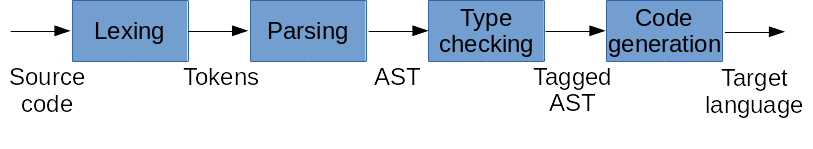
\includegraphics[width=\columnwidth]{./compiler_pipeline.png}
\caption{A classic compiler pipeline}
\label{fig:compiler_pipeline}
\end{figure}

The compiler described in this paper also uses a pipeline approach, but with different steps (see figure \ref{fig:pack.hs_pipeline}).

\begin{figure}[H]
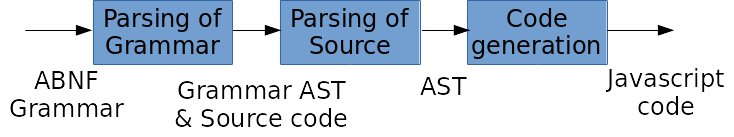
\includegraphics[width=\columnwidth]{./pack_hs_pipeline.png}
\caption{A classic compiler pipeline}
\label{fig:pack.hs_pipeline}
\end{figure}

